% ======================================================================
% scrjura-de.tex
% Copyright (c) Markus Kohm, 2011-2023
%
% This file is part of the LaTeX2e KOMA-Script bundle.
%
% This work may be distributed and/or modified under the conditions of
% the LaTeX Project Public License, version 1.3c of the license.
% The latest version of this license is in
%   http://www.latex-project.org/lppl.txt
% and version 1.3c or later is part of all distributions of LaTeX 
% version 2005/12/01 or later and of this work.
%
% This work has the LPPL maintenance status "author-maintained".
%
% The Current Maintainer and author of this work is Markus Kohm.
%
% This work consists of all files listed in MANIFEST.md.
% ======================================================================
%
% Chapter about scrjura of the KOMA-Script guide
% Maintained by Markus Kohm
%
% ======================================================================

\KOMAProvidesFile{scrjura-de.tex}%
                 [$Date: 2023-04-16 13:50:16 +0200 (So, 16. Apr 2023) $
                  KOMA-Script guide (chapter: scrjura)]

\chapter{Unterstützung für die Anwaltspraxis durch \Package{scrjura}}
\labelbase{scrjura}
\BeginIndexGroup
\BeginIndex{Package}{scrjura}

Will man einen Vertrag\Index{Vertraege=Verträge}, die Satzung einer
Gesellschaft oder eines Vereins, ein Gesetz oder gleich einen
Gesetzeskommentar schreiben, so übernimmt das Paket \Package{scrjura} den
typografischen Teil der Unterstützung für diese Tätigkeit. Obwohl
\Package{scrjura} als allgemeine Hilfe für anwaltliche Schriftstücke angedacht
ist, hat sich gezeigt, dass der Vertrag dabei ein ganz zentrales Element
ist. Besonderes Augenmerk gilt hier dem
Paragraphen\Index{Paragraphen>juristische} mit Nummer, Titel, nummerierten
Absätzen -- falls es mehrere davon in einem Paragraphen gibt --, bedarfsweise
nummerierten Sätzen, Einträgen in das Inhaltsverzeichnis und Querverweisen in
den deutschen Gepflogenheiten entsprechenden Formen.

Das Paket ist in Zusammenarbeit mit Rechtsanwalt Dr.\,Alexander Willand,
Karlsruhe, entstanden. Viele der Möglichkeiten gehen außerdem auf konstruktive
Nachfragen von Prof.\,Heiner Richter von der Hochschule Stalsund zurück.

\iffalse % Umbruchkorrektur
Es ist zu beachten, dass das Paket mit
\Package{hyperref}\IndexPackage{hyperref}\important{\Package{hyperref}}
zusammenarbeitet. %
\else%
Das Paket arbeitet auch mit
\Package{hyperref}\IndexPackage{hyperref}\important{\Package{hyperref}}
zusammen. %
\fi%
Es ist dabei jedoch wichtig, dass \Package{hyperref} wie üblich nach
\Package{scrjura} geladen wird!

\LoadCommonFile{options}% \section{Frühe oder späte Optionenwahl}

\LoadCommonFile{textmarkup}% \section{Textauszeichnungen} 

\section{Verzeichnisse}
\seclabel{toc}

Die Überschriften juristischer Paragraphen können auf Wunsch automatisch
ins Inhaltsverzeichnis eingetragen
werden. Dazu\ChangedAt{v3.27}{\Package{scrjura}} definiert das Paket mit Hilfe
von \DescRef{tocbasic.cmd.DeclareTOCStyleEntry} (siehe
\autoref{sec:tocbasic.tocstyle} ab
\DescPageRef{tocbasic.cmd.DeclareTOCStyleEntry})\IndexCmd{DeclareTOCStyleEntry}
die Verzeichnisebene \PValue{cpar}.

\begin{Declaration}
  \OptionVName{juratotoc}{Ein-Aus-Wert}
  \OptionVName{juratotoc}{Ebenennummer}
\end{Declaration}
Im Inhaltsverzeichnis angezeigt werden
Paragraphen\Index{Paragraphen>juristische} nur, wenn ihre \PName{Ebenennummer}
kleiner oder gleich dem Zähler \DescRef{maincls.counter.tocdepth}%
\important{\DescRef{maincls.counter.tocdepth}}\IndexCounter{tocdepth} ist
(siehe \autoref{sec:maincls.toc},
\DescPageRef{maincls.counter.tocdepth}). Voreingestellt\textnote{Voreinstellung}
ist für \PName{Ebenennummer} der Wert \Length{maxdimen}, der auch verwendet
wird, wenn die Option über einen
\PName{Ein-Aus-Wert}\important{\OptionValue{juratotoc}{false}} (siehe
\autoref{tab:truefalseswitch}, \autopageref{tab:truefalseswitch})
ausgeschaltet wird. Da der Zähler \DescRef{maincls.counter.tocdepth}
üblicherweise einen kleinen, einstelligen Wert besitzt, werden die
Paragraphen-Einträge im Inhaltsverzeichnis daher normalerweise nicht
angezeigt.

Wird die Option hingegen über einen
\PName{Ein-Aus-Wert}\important{\OptionValue{juratotoc}{true}} eingeschaltet,
so wird als \PName{Ebenennummer} 2 voreingestellt. Damit werden sie in
Inhaltsverzeichnissen bei allen \KOMAScript-Klassen auf derselben Ebene wie
\DescRef{maincls.cmd.subsection}\IndexCmd{subsection}%
\important{\DescRef{maincls.cmd.subsection}} eingeordnet. In der
Voreinstellung von \DescRef{maincls.counter.tocdepth} werden sie dann auch bei
allen \KOMAScript-Klassen im Inhaltsverzeichnis angezeigt.

Intern\ChangedAt{v3.27}{\Package{scrjura}} führt die Verwendung der Option zu
einem erneuten Aufruf von
\DescRef{tocbasic.cmd.DeclareTOCStyleEntry}\IndexCmd{DeclareTOCStyleEntry}
mit dem \PName{Stil} \PValue{default} und entsprechender Einstellung für
\Option{level} in der \PName{Optionenlist}.%
\EndIndexGroup


\begin{Declaration}
  \OptionVName{juratocindent}{Einzug}
  \OptionVName{juratocnumberwidth}{Nummernbreite}
\end{Declaration}
Mit diesen beiden Optionen kann für die Einträge der Paragraphen ins
Inhaltsverzeichnis sowohl der Einzug als auch die Breite, die für Nummern
reserviert wird, festgelegt werden. Voreingestellt\textnote{Voreinstellung}
sind dieselben Werte wie für
\DescRef{maincls.cmd.subsection}-Einträge\IndexCmd{subsection}%
\important{\DescRef{maincls.cmd.subsection}} bei \Class{scrartcl}, also
\OptionValue{juratocindent}{1.5em} und \OptionValue{juratocnumberwidth}{2em}.

Intern\ChangedAt{v3.27}{\Package{scrjura}} führt die Verwendung der Optionen
zu einem erneuten Aufruf von
\DescRef{tocbasic.cmd.DeclareTOCStyleEntry}\IndexCmd{DeclareTOCStyleEntry} mit
dem \PName{Stil} \PValue{default} und \OptionVName{indent}{Einzug}
beziehungsweise \OptionVName{numwidth}{Nummernbreite} in der
\PName{Optionenlist}.%
\EndIndexGroup


\section{Umgebung für Verträge}
\seclabel{contract}

\BeginIndexGroup
\BeginIndex{}{Vertraege=Verträge}
Die wesentlichen Mechanismen von \Package{scrjura} stehen ausschließlich
innerhalb von Verträgen der zugehörigen Umgebung zur Verfügung.

\begin{Declaration}
  \begin{Environment}{contract}\end{Environment}
\end{Declaration}
Dies ist die erste und bisher einzige Umgebung für Juristen, die
\Package{scrjura} bereitstellt. Durch ihre Verwendung wird die automatische
Absatznummerierung aktiviert und die Anweisungen
\DescRef{\LabelBase.cmd.Clause} und \DescRef{\LabelBase.cmd.SubClause} mit
einer konkreten Form versehen, die später näher dokumentiert wird.

Die\textnote{Achtung!} Umgebung \Environment{contract} darf nicht in sich
selbst geschachtelt werden. Innerhalb eines Dokuments dürfen jedoch mehrere
dieser Umgebungen verwendet werden. Dabei werden die Paragraphen innerhalb
dieser Umgebungen so behandelt, als stünden sie innerhalb einer einzigen
Umgebung. Durch das Beenden der Umgebung wird diese also quasi
unterbrochen und durch den Beginn einer neuen Umgebung wird sozusagen die alte
Umgebung fortgesetzt. Dabei sind allerdings keine Unterbrechungen innerhalb
eines Paragraphen möglich.

Sollten Sie stattdessen Umgebungen für voneinander unabhängige Verträgen
innerhalb desselben Dokuments benötigen, so sei auf die Möglichkeit der
Definition weiterer Vertragsumgebungen mit
\DescRef{\LabelBase.cmd.DeclareNewJuraEnvironment} in
\autoref{sec:\LabelBase.newenv},
\DescPageRef{\LabelBase.cmd.DeclareNewJuraEnvironment}) verwiesen.%
\EndIndexGroup

\begin{Declaration}
  \Option{contract}
\end{Declaration}
Durch Angabe dieser Option beim Laden des Pakets, beispielsweise mit
\DescRef{\LabelBase.cmd.usepackage}%
\important{\DescRef{\LabelBase.cmd.usepackage}} oder als globale Option bei
\DescRef{\LabelBase.cmd.documentclass}%
\important{\DescRef{\LabelBase.cmd.documentclass}}, wird das gesamte Dokument
zu einem Vertrag. Das Dokument verhält sich dann also genauso, als würde es
genau eine \DescRef{\LabelBase.env.contract}-Umgebung enthalten.

Es\textnote{Achtung!} wird darauf hingewiesen, dass Option \Option{contract}
weder mit \DescRef{\LabelBase.cmd.KOMAoption} noch
\DescRef{\LabelBase.cmd.KOMAoptions} gesetzt werden kann!  Damit ist es auch
nicht möglich die Option wieder abzuschalten. Außerdem würde mit der Option
beispielsweise ein Dokumenttitel innerhalb der Vertragsumgebung
gesetzt werden, was zu vermeiden ist. Verwenden Sie in solchen Fällen
besser eine explizite \DescRef{\LabelBase.env.contract}-Umgebung.%
\EndIndexGroup


\subsection{Juristische Paragraphen}
\label{sec:scrjura.clause}
\BeginIndexGroup
\BeginIndex{}{Paragraphen>juristische} 

Paragraphen im juristischen Sinn sind bei \Package{scrjura} nur innerhalb von
Verträgen, also innerhalb der Umgebung \DescRef{\LabelBase.env.contract} oder
weiteren mit \DescRef{\LabelBase.cmd.DeclareNewJuraEnvironment} (siehe
\autoref{sec:\LabelBase.newenv},
\DescPageRef{\LabelBase.cmd.DeclareNewJuraEnvironment}) erstellten Umgebungen,
definiert. Um Verwechslungen\textnote{Hinweis!} von juristischen Paragraphen
mit Gliederungsbefehlen für typografische Paragraphen oder Abschnitte zu
vermeiden, leiten sich die Bezeichnungen von \Package{scrjura} nicht vom dem
eigentlich korrekten englischen Begriff »\emph{section}«, sondern von
»\emph{clause}« ab.

\begin{Declaration}
  \phantomsection\label{desc:scrjura.contract.macro.Clause}%
  \Macro{Clause}\Parameter{Einstellungen}
  \phantomsection\label{desc:scrjura.contract.macro.SubClause}%
  \Macro{SubClause}\Parameter{Einstellungen}
\end{Declaration}
Dies sind die wichtigsten Anweisungen innerhalb eines Vertrags. Ohne
zusätzliche \PName{Einstellungen} erzeugt \Macro{Clause} eine
Paragraphenüberschrift, die nur aus dem Paragraphenzeichen, gefolgt von einer
fortlaufenden Nummer besteht. Dagegen erzeugt \Macro{SubClause} eine
Paragraphenüberschrift, bei der an die zuletzt mit \Macro{Clause} gesetzte
Nummer noch ein fortlaufender Kleinbuchstabe angehängt wird. Gedacht ist
\Macro{SubClause} vor allem für den Fall, dass bei der Novellierung von
Gesetzen oder Verträgen nicht nur Paragraphen umformuliert oder gestrichen
werden, sondern zwischen existierenden Paragraphen neue eingefügt werden, ohne
dass eine komplett neue Nummerierung erfolgt. Bezüglich der generellen
Formatierung oder beispielsweise der Erzeugung von Inhaltsverzeichniseinträgen
wird jedoch nicht zwischen \Macro{Clause} und \Macro{SubClause} unterschieden.

Als \PName{Einstellungen} kann bei beiden Anweisungen eine durch Komma
separierte Liste von Eigenschaften angegeben werden. Eine Übersicht über die
möglichen Eigenschaften bietet \autoref{tab:scrjura.Clause.options}. Auf die
wichtigsten soll noch näher eingegangen werden.%
\begin{table}
  \caption{Mögliche Eigenschaften für die optionalen Argumente der Anweisungen
    \Macro{Clause} und \Macro{SubClause}}
  \label{tab:scrjura.Clause.options}
  \begin{desctabular}
    \entry{\Option{dummy}}{%
      Die Überschrift wird nicht gesetzt, aber gezählt.%
    }\\[-1.7ex]
    \entry{\OptionVName{head}{Kolumnentitel}}{%
      Sind Kolumnentitel aktiviert, wird unabhängig von einem Titel für den
      Paragraphen dieser Kolumnentitel verwendet.%
    }\\[-1.7ex]
    \entry{\Option{nohead}}{%
      Es wird kein neuer Kolumnentitel gesetzt.%
    }\\[-1.7ex]
    \entry{\Option{notocentry}}{%
      Es wird kein Eintrag ins Inhaltsverzeichnis vorgenommen.%
    }\\[-1.7ex]
    \entry{\OptionVName{number}{Nummer}}{%
      Die Nummer für den Paragraphen wird direkt angegeben.%
    }\\[-1.7ex]
    \entry{\OptionVName{preskip}{Abstand}}{%
      Neuer Abstand vor den Überschriften der Paragraphen.%
    }\\[-1.7ex]
    \entry{\OptionVName{postskip}{Abstand}}{%
      Neuer Abstand nach den Überschrift der Paragraphen.%
    }\\[-1.7ex]
    \entry{\OptionVName{title}{Überschrift}}{%
      Der Paragraph wird zusätzlich zur Nummer mit einem Titel versehen. Dies
      ist gleichzeitig die Grundeinstellung für die Einträge in den
      Kolumnentitel und das Inhaltsverzeichnis.%
    }\\[-1.7ex]
    \entry{\OptionVName{tocentry}{Inhaltsverzeichniseintrag}}{%
      Unabhängig von einem Titel für den Paragraphen wird dieser Eintrag ins
      Inhaltsverzeichnis vorgenommen.%
    }%
  \end{desctabular} 
\end{table}

In der Voreinstellung\textnote{Voreinstellung} wird vor der Überschrift ein
Abstand von zwei Zeilen und danach ein Abstand von einer Zeile eingefügt. Über
die Eigenschaften \Option{preskip}\important[i]{\Option{preskip},
  \Option{postskip}} und \Option{postskip} kann dieser Abstand verändert
werden. Die neue Einstellung gilt dann aber nicht nur für den aktuellen
Paragraphen, sondern ab dem aktuellen Paragraphen bis zum Ende der aktuellen
Umgebung. Es ist auch möglich, die entsprechende Einstellung bereits vorab mit
Hilfe von
\begin{lstcode}[escapeinside=><]
  \setkeys{contract}{preskip=>\PName{Abstand}<,postskip=>\PName{Abstand}<}
\end{lstcode}
unabhängig von einem konkreten Paragraphen, außerhalb einer
\DescRef{\LabelBase.env.contract}-Umgebung vorzunehmen. Auch das Setzen
innerhalb der Präambel nach dem Laden von \Package{scrjura} ist so
möglich. Dagegen ist es nicht möglich, diese beiden Optionen bereits beim
Laden des Pakets anzugeben oder sie per \DescRef{\LabelBase.cmd.KOMAoptions}
oder \DescRef{\LabelBase.cmd.KOMAoption} zu setzen.

\BeginIndex{FontElement}{contract.Clause}\LabelFontElement{contract.Clause}%
\BeginIndex{FontElement}{Clause}\LabelFontElement{Clause}%
In der Voreinstellung\textnote{Voreinstellung} wird für die Überschrift des
Paragraphen als Schrift \Macro{sffamily}\Macro{bfseries}\Macro{large}
verwendet. Über das Element
\FontElement{contract.Clause}\important{\FontElement{contract.Clause}} kann
diese Schrift jederzeit mit Hilfe der Anweisungen
\DescRef{\LabelBase.cmd.setkomafont}%
\important[i]{\DescRef{\LabelBase.cmd.setkomafont},
  \DescRef{\LabelBase.cmd.addtokomafont}} und
\DescRef{\LabelBase.cmd.addtokomafont} (siehe
\autoref{sec:\LabelBase.textmarkup}, \DescPageRef{\LabelBase.cmd.setkomafont})
geändert werden. Innerhalb der \DescRef{\LabelBase.env.contract}-Umgebung kann
statt \FontElement{contract.Clause} auch
\FontElement{Clause}\important{\FontElement{Clause}} verwendet werden.%
\EndIndex{FontElement}{Clause}%
\EndIndex{FontElement}{contract.Clause}

Mit Hilfe der Einstellungen \Option{title}\important[i]{\Option{title},
  \Option{head}, \Option{tocentry}}, \Option{head} und \Option{tocentry}
können Paragraphen zusätzlich zur Nummer mit einem Titel versehen
werden. Dabei\textnote{Achtung!} wird empfohlen, den Wert der jeweiligen
Eigenschaft in geschweifte Klammern zu setzen. Anderenfalls führen
beispielsweise Kommata zu Verwechslungen mit den Trennzeichen zwischen
unterschiedlichen Eigenschaften. Leere Werte für \Option{head} und
\Option{tocentry} führen zu leeren Einträgen. Will man hingegen keine Einträge
vornehmen, so sind \Option{nohead}\important[i]{\Option{nohead},
  \Option{notocentry}} und \Option{notocentry} zu verwenden.

Statt der fortlaufenden Nummer kann mit Hilfe der Eigenschaft
\Option{number}\important{\Option{number}} auch manuell eine Nummer vergeben
werden. Dies hat jedoch keinen Einfluss auf die Nummern der nachfolgenden
Paragraphen. Die Angabe einer leeren Nummer ist nicht
vorgesehen. Zerbrechliche Anweisungen in \PName{Nummer} sollten mit
\Macro{protect} geschützt werden. Es\textnote{Achtung!} wird empfohlen als
\PName{Nummer} nur Ziffern und Buchstaben anzugeben.

Mit der Eigenschaft \Option{dummy}\important{\Option{dummy}} kann man die
Ausgabe der kompletten Überschrift des Paragraphen unterdrücken. In der
automatischen Zählung wird der Paragraph aber dennoch berücksichtigt. Auf
diese Weise kann man beispielsweise\textnote{Beispiel} mit
\begin{lstcode}
  \Clause{dummy}
\end{lstcode}
einen Paragraphen in der automatischen Zählung überspringen, falls der
entsprechende Paragraph in einer späteren Fassung eines Vertrags gestrichen
wurde.

Es\textnote{Achtung!} ist zu beachten, dass die Eigenschaft \Option{dummy} als
Wert allenfalls \PValue{true} und \PValue{false} versteht. Andere Werte
können zu einer Fehlermeldung führen.%
\EndIndexGroup


\begin{Declaration}
  \Macro{Clauseformat}\Parameter{Nummer}
\end{Declaration}
Wie bereits in der vorausgehenden Erklärung erwähnt, werden juristische
Paragraphen und Unterparagraphen normalerweise nummeriert. Die Formatierung
der Nummer erfolgt dabei mit Hilfe der Anweisung \Macro{Clauseformat}, die als
einziges Argument die Nummer erwartet. Bei der
Vordefinierung\textnote{Voreinstellung} als
\begin{lstcode}
  \newcommand*{\Clauseformat}[1]{\S~#1}
\end{lstcode}
wird der Nummer mit \Macro{S}\IndexCmd{S} lediglich das Paragraphensymbol,
gefolgt von einem nicht trennbaren Leerzeichen
vorangestellt. Bei\textnote{Achtung!}  Umdefinierungen ist auf die
Expandierbarkeit zu achten!%
\EndIndexGroup


\begin{Declaration}
  \OptionVName{juratitlepagebreak}{Ein-Aus-Wert}
\end{Declaration}%
Normalerweise sind Seitenumbrüche innerhalb von Überschriften aller Art
verboten. Einige Juristen benötigen jedoch Seitenumbrüche innerhalb von
Paragraphentiteln. Daher kann ein solcher Umbruch mit
\Option{juratitlepagebreak}\important{\Option{juratitlepagebreak}} erlaubt
werden. Die möglichen Einstellungen für \PName{Ein-Aus-Wert} sind
\autoref{tab:truefalseswitch}, \autopageref{tab:truefalseswitch} zu
entnehmen.

Bitte beachten Sie\textnote{Achtung!}, dass es sich hier nicht um eine Option
für \DescRef{\LabelBase.cmd.Clause} oder \DescRef{\LabelBase.cmd.SubClause},
sondern um eine \KOMAScript-Option handelt. Außer beim Laden des Pakets kann
sie auch jederzeit mit \DescRef{\LabelBase.cmd.KOMAoptions} oder
\DescRef{\LabelBase.cmd.KOMAoption} geändert werden und gilt dann bis zum Ende
der aktuellen Umgebung.%
\EndIndexGroup

  
\begin{Declaration}
  \OptionVName{clausemark}{Einstellung}
\end{Declaration}%
Da Paragraphen eine untergeordnete Gliederung mit unabhängiger Nummerierung
sind, erzeugen sie in der Voreinstellung\textnote{Voreinstellung} keine
Kolumnentitel. Über alternative Einstellungen können jedoch auch Kolumnentitel
erzeugt werden. Die möglichen Werte und ihre Bedeutung sind
\autoref{tab:scrjura.clausemark} zu entnehmen.%
%
\begin{table}
  \caption{Mögliche Werte für Option \Option{clausemark} zur Erzeugung von
    Kolumnentiteln durch Paragraphen}
  \label{tab:scrjura.clausemark}%
  \begin{desctabular}
    \entry{\PValue{both}}{%
      Paragraphen erzeugen linke und rechte Marken für Kolumnentitel, wenn das
      Dokument die Verwendung von lebenden Kolumnentiteln vorsieht.%
      \IndexOption{clausemark~=\textKValue{both}}%
    }\\[-1.7ex]
    \entry{\PValue{false}, \PValue{off}, \PValue{no}}{%
      Paragraphen erzeugen keine Kolumnentitel.%
      \IndexOption{clausemark~=\textKValue{false}}%
    }\\[-1.7ex]
    \entry{\PValue{forceboth}}{%
      Paragraphen erzeugen mit \DescRef{maincls.cmd.markboth} linke und rechte
      Marken für Kolumnentitel unabhängig davon, ob das Dokument
      beispielsweise über den Seitenstil überhaupt lebende Kolumnentitel
      verwendet.%
      \IndexOption{clausemark~=\textKValue{forceboth}}%
    }\\[-1.7ex]
    \entry{\PValue{forceright}}{%
      Paragraphen erzeugen mit \DescRef{maincls.cmd.markright} rechte Marken
      für Kolumnentitel unabhängig davon, ob das Dokument beispielsweise über
      den Seitenstil überhaupt lebende Kolumnentitel verwendet.%
      \IndexOption{clausemark~=\textKValue{forceright}}%
    }\\[-1.7ex]
    \entry{\PValue{right}}{%
      Paragraphen erzeugen rechte Marken für Kolumnentitel, wenn das Dokument
      die Verwendung von lebenden Kolumnentiteln vorsieht.%
      \IndexOption{clausemark~=\textKValue{right}}%
    }%
  \end{desctabular}
\end{table}

Bitte beachten Sie\textnote{Achtung!}, dass es sich hier nicht um eine Option
für \DescRef{\LabelBase.cmd.Clause} oder \DescRef{\LabelBase.cmd.SubClause},
sondern um eine \KOMAScript-Option handelt. Außer beim Laden des Pakets kann
sie auch jederzeit mit \DescRef{\LabelBase.cmd.KOMAoptions} oder
\DescRef{\LabelBase.cmd.KOMAoption} geändert werden und gilt dann bis zum Ende
der aktuellen Umgebung.%
\EndIndexGroup \EndIndexGroup

\subsection{Absätze}
\label{sec:scrjura.par}
\BeginIndexGroup
\BeginIndex{}{Absatz>Nummerierung}%
Innerhalb von Paragraphen werden Absätze von \Package{scrjura} normalerweise
automatisch nummeriert. Sie sind damit ein stark gliederndes Element, ähnlich
\DescRef{maincls.cmd.paragraph} oder \DescRef{maincls.cmd.subparagraph} in
normalen Texten. Innerhalb von Verträgen wird deshalb häufig auch gerne mit
Abstand zwischen den Absätzen gearbeitet. Das Paket \Package{scrjura} bietet
keinen eigenen Mechanismus hierfür. Stattdessen sei auf die Option
\DescRef{maincls.option.parskip}%
\IndexOption{parskip}\important{\DescRef{maincls.option.parskip}} der
\KOMAScript-Klassen verwiesen (siehe \autoref{sec:maincls.parmarkup},
\DescPageRef{maincls.option.parskip}).

\begin{Declaration}
  \OptionVName{parnumber}{Einstellung}
\end{Declaration}
Die automatische\textnote{Voreinstellung} Nummerierung der Absätze entspricht
den beiden Einstellungen \OptionValue{parnumber}{auto} und
\OptionValue{parnumber}{true}. Manchmal ist es notwendig, die automatische
Nummerierung abzuschalten. Das ist mit \OptionValue{parnumber}{false}%
\important{\OptionValue{parnumber}{false}}%
\IndexOption{parnumber~=\textKValue{false}} möglich. In diesem Fall wird nur die
Satznummer automatisch zurückgesetzt.

Zur Realisierung dieser Option war es notwendig, in den Absatzmechanismus von
\LaTeX{} einzugreifen. In einigen seltenen Fällen kann sich das negativ
auswirken. Dann bleibt nur, diese Änderung mit
\OptionValue{parnumber}{manual}%
\important{\OptionValue{parnumber}{manual}}%
\IndexOption{parnumber~=\textKValue{manual}} zurückzunehmen. Umgekehrt hebt
\LaTeX{} selbst den Eingriff manchmal auf. In diesem Fällen kann er mit
\OptionValue{parnumber}{auto}%
\important{\OptionValue{parnumber}{auto}}%
\IndexOption{parnumber~=\textKValue{auto}} erneut aktiviert werden.

Paragraphen, die nur aus einem einzigen Absatz bestehen, werden normalerweise
nicht automatisch nummeriert. Damit dies funktioniert, dürfen sich keine zwei
Paragraphen mit identischer Nummer in einem Dokument befinden. Sollten Sie
dies dennoch einmal benötigen, weichen Sie bitte auf eine weitere
Vertragsumgebung aus (siehe
\DescRef{\LabelBase.cmd.DeclareNewJuraEnvironment},
\autoref{sec:\LabelBase.newenv},
\DescPageRef{\LabelBase.cmd.DeclareNewJuraEnvironment}). Da\textnote{Achtung!}
die Information erst am Ende eines Paragraphen zur Verfügung steht, werden in
der Regel zwei \LaTeX-Läufe benötigt, bis die automatische Absatznummerierung
korrekt erfolgt.%
\EndIndexGroup

\begin{Declaration}
  \Counter{par}
  \Macro{thepar}
  \Macro{parformat}
  \Macro{parformatseparation}
\end{Declaration}%
Für die Nummerierung der Absätze wird der Zähler \Counter{par}
verwendet. Seine Darstellung \Macro{thepar} ist mit
\Macro{arabic}\PParameter{par} als arabische Zahl
voreingestellt. Die\textnote{Voreinstellung} Ausgabe als automatische
Absatznummer erfolgt mit \Macro{parformat}. Dabei wird \Macro{thepar} in runde
Klammern gesetzt. Will man einem Absatz manuell eine Absatznummer
voranstellen, so sollte das ebenfalls mit \Macro{parformat} geschehen. Dabei
ist es sinnvoll, auf \Macro{parformat} noch \Macro{parformatseparation} oder
zumindest ein nicht trennbares Leerzeichen mit
\Macro{nobreakspace}\IndexCmd{nobreakspace} oder der Tilde folgen zu lassen.

Bei\ChangedAt{v0.7}{\Package{scrjura}} der automatischen Nummerierung wird
\Macro{parformat} ebenfalls noch \Macro{parformatseparation} als Trennzeichen
angehängt. Voreinstellt\textnote{Voreinstellung} ist derzeit mit
\Macro{nobreakspace}\IndexCmd{nobreakspace} ein nicht umbrechbarer
Wortabstand.

\BeginIndex{FontElement}{parnumber}\LabelFontElement{parnumber}%
Die Absatznummer wird normalerweise\textnote{Voreinstellung} in der
aktuellen Schrift gesetzt. Diese Voreinstellung für das Element
\FontElement{parnumber} kann jederzeit mit Hilfe der Anweisungen
\DescRef{\LabelBase.cmd.setkomafont}%
\important[i]{\DescRef{\LabelBase.cmd.setkomafont},
  \DescRef{\LabelBase.cmd.addtokomafont}} und
\DescRef{\LabelBase.cmd.addtokomafont} (siehe
\autoref{sec:\LabelBase.textmarkup}, \DescPageRef{\LabelBase.cmd.setkomafont})
geändert werden.%
\EndIndex{FontElement}{parnumber}%

Es\textnote{Achtung!} wird darauf hingewiesen, dass \Package{scrjura} intern
davon ausgeht, dass \Macro{thepar} eine arabische Zahl ist. Daher sollte
diese Anweisung keinesfalls umdefiniert werden!%
\EndIndexGroup


\begin{Declaration}
  \Macro{withoutparnumber}
\end{Declaration}
Wird keine Absatznummer ausgegeben, wird am Anfang des Absatzes ersatzweise
die Anweisung \Macro{withoutparnumber} lokal
ausgeführt. Diese\textnote{Voreinstellung} ist in der Voreinstellung leer, tut
also weiter nichts. Sie wurde auf speziellen Wunsch in \Package{scrjura}
eingebaut, ist für den normalen Anwender aber ohne Belang.%
\EndIndexGroup


\begin{Declaration}
  \Macro{ellipsispar}\OParameter{Anzahl}
  \Macro{parellipsis}
\end{Declaration}
Manchmal\ChangedAt{v0.7}{\Package{scrjura}} -- insbesondere in vergleichenden
Kommentaren -- ist es wünschenswert, wenn man Absätze in Gesetzen auslassen,
aber gleichzeitig die Auslassung\Index{Absatz>Auslassung} markieren kann. Die
Absätze sollen dann auch in der Zählung der übrigen Absätze berücksichtigt
werden. Das Paket \Package{scrjura} stellt dafür die Anweisung
\Macro{ellipsispar} bereit. 

In der Voreinstellung\textnote{Voreinstellung} lässt \Macro{ellipsispar} genau
einen Absatz aus. Über das optionale Argument \PName{Anzahl} können jedoch
auch mehrere Absätze ausgelassen werden. In jedem Fall erscheint in der
Ausgabe stattdessen genau ein nicht nummerierter Absatz, der nur die
Auslassungszeichen \Macro{parellipsis} enthält. Bei der Entscheidung für eine
automatische Nummerierung der übrigen Absätze eines juristischen Paragraphen
werden die ausgelassenen Absätze jedoch mitgezählt. Dies gilt ebenso für die
Nummern etwaiger nachfolgender Absätze.
\begin{Example}
  Angenommen, Sie kommentieren das Strafgesetzbuch, wollen aber in \S~2 nur
  Absatz~3 kommentieren. Dennoch soll auf die übrigen Absätze indirekt
  hingewiesen werden. Sie erreichen das beispielsweise mit:
\begin{lstcode}
  \documentclass[parskip=half]{scrartcl}
  \usepackage{scrjura}
  \begin{document}
  \begin{contract}
    \Clause{title={Zeitliche Geltung},number=2}
    \ellipsispar[2]

    Wird das Gesetz, das bei Beendigung der Tat
    gilt, vor der Entscheidung geändert, so ist
    das mildeste Gesetz anzuwenden.

    \ellipsispar[3]
  \end{contract}
  \end{document}
\end{lstcode}
  Wenn\textnote{Achtung!} Sie dieses Beispiel ausprobieren wollen, verwenden
  Sie bitte eine \LaTeX-Version ab 2018-04-01 und einen Editor mit der
  Codierungseinstellung UTF-8. Dies ist bei aktuellen \TeX-Distributionen und
  aktuellen \LaTeX-Editoren die Voreinstellung. Bei Verwendung einer
  veralteten \TeX-Distribution oder einer anderen Einstellung des Editor,
  müssen Sie die verwendete Codierung mit Hilfe des Pakets
  \Package{inputenc}\IndexPackage{inputenc} deklarieren.%
\end{Example}

Die Auslassungszeichen sind so vordefiniert\textnote{Voreinstellung}, dass
\Macro{textellipsis}\IndexCmd{textellipsis} verwendet wird, falls eine solche
Anweisung definiert ist. Anderenfalls wird \Macro{dots}\IndexCmd{dots}
verwendet. Eine Umdefinierung von \Macro{parellipsis} ist mit
\Macro{renewcommand} jederzeit möglich.%
\EndIndexGroup


\subsection{Sätze}
\label{sec:scrjura.sentence}

\BeginIndexGroup%
\BeginIndex{}{Satz>Nummerierung}%
Absätze in Verträgen bestehen aus einem oder mehreren Sätzen, die teilweise
ebenfalls nummeriert werden. Da eine automatische Nummerierung problematisch
und fehleranfällig ist, wird nur eine halbautomatische Nummerierung
unterstützt.

\begin{Declaration}
  \Counter{sentence}
  \Macro{thesentence}
  \Macro{sentencenumberformat}
  \Macro{Sentence}
\end{Declaration}
Die Nummerierung von Sätzen erfolgt manuell mit der Anweisung
\Macro{Sentence}. Dabei wird der Zähler \Counter{sentence} automatisch erhöht
und in der Voreinstellung von
\Macro{sentencenumberformat}\ChangedAt{v3.26}{\Package{scrjura}} die arabische
Zahl von \Macro{thesentence} hochgestellt ausgegeben.

\BeginIndex{FontElement}{sentencenumber}\LabelFontElement{sentencenumber}%
Die\ChangedAt{v3.26}{\Package{scrjura}} Satznummer wird
normalerweise\textnote{Voreinstellung} in der aktuellen Schrift gesetzt. Diese
Voreinstellung für das Element \FontElement{sentencenumber} kann mit
Hilfe der Anweisungen \DescRef{\LabelBase.cmd.setkomafont}%
\important[i]{\DescRef{\LabelBase.cmd.setkomafont},
  \DescRef{\LabelBase.cmd.addtokomafont}} und
\DescRef{\LabelBase.cmd.addtokomafont} (siehe
\autoref{sec:\LabelBase.textmarkup}, \DescPageRef{\LabelBase.cmd.setkomafont})
geändert werden.%
\EndIndex{FontElement}{sentencenumber}

Bei\textnote{Tipp!} Verwendung von Paket
\Package{babel}\IndexPackage{babel}\important{\Package{babel}} ist es einfach
möglich, eine Abkürzung für \Macro{Sentence} zu definieren:%
\phantomsection\label{sec:scrjura.shorthandexample}%
\begin{lstcode}[moretexcs={useshorthands,defineshorthand}]
  \useshorthands{'}
  \defineshorthand{'S}{\Sentence\ignorespaces}
\end{lstcode}
Dabei werden Leerzeichen nach
\lstinline|'S| ignoriert. Auch eine
Abkürzung für einen Punkt, gefolgt von einer neuen Satznummer ist möglich:
\begin{lstcode}[moretexcs={useshorthands,defineshorthand}]
  \defineshorthand{'.}{. \Sentence\ignorespaces}
\end{lstcode}
Näheres zu \Macro{useshorthands}\IndexCmd{useshorthands} und
\Macro{defineshorthand}\IndexCmd{defineshorthands} ist der Anleitung zum Paket
\Package{babel} zu entnehmen (siehe \cite{package:babel}). Ein
Anwendungsbeispiel finden Sie in \autoref{sec:scrjura.example} ab
\autopageref{sec:scrjura.example}.%
\EndIndexGroup
%
\EndIndexGroup
%
\EndIndexGroup
%
\EndIndexGroup


\section{Querverweise}
\seclabel{ref}

Für Paragraphen, Absätze und Sätze reicht der normale Mechanismus für
Querverweise mit \Macro{label}\IndexCmd{label}\important{\Macro{label}},
\Macro{ref} und \Macro{pageref} nicht mehr aus. Daher wird dieser von
\Package{scrjura} um weitere Anweisungen ergänzt.

\begin{Declaration}
  \Macro{ref}\Parameter{Label}
  \Macro{refL}\Parameter{Label}
  \Macro{refS}\Parameter{Label}
  \Macro{refN}\Parameter{Label}
\end{Declaration}
Die Anweisungen \Macro{refL}, \Macro{refS} und \Macro{refN}
referenzieren Paragraph, Absatz und Satz immer vollständig. \Macro{refL}
verwendet dabei eine textuelle Langform, während \Macro{refS} eine textuelle
Kurzform bietet. \Macro{refN} ist eine rein numerische Kurzform. \Macro{ref}
entspricht in der Voreinstellung\textnote{Voreinstellung} \Macro{refL}.%
\EndIndexGroup


\begin{Declaration}
  \Macro{refSentence}\Parameter{Label}
  \Macro{refSentenceL}\Parameter{Label}
  \Macro{refSentenceS}\Parameter{Label}
  \Macro{refSentenceN}\Parameter{Label}
\end{Declaration}
Der Satz ohne Paragraph und Absatz kann mit \Macro{refSentenceL},
\Macro{refSentenceS} oder \Macro{refSentenceN} referenziert werden. Auch hier
gibt es wieder eine textuelle Langform, eine textuelle Kurzform und eine rein
numerische Form. \Macro{refSentence} entspricht in der
Voreinstellung\textnote{Voreinstellung} \Macro{refSentenceL}.%
\EndIndexGroup


\begin{Declaration}
  \Macro{refPar}\Parameter{Label}
  \Macro{refParL}\Parameter{Label}
  \Macro{refParS}\Parameter{Label}
  \Macro{refParN}\OParameter{Zahlenformat}\Parameter{Label}
\end{Declaration}
Nur den Absatz kann man mit \Macro{refParL}, \Macro{refParS} und
\Macro{refParN} referenzieren. Die Formen unterscheiden sich dabei wie bereits
für \DescRef{\LabelBase.cmd.refL}, \DescRef{\LabelBase.cmd.refN} und
\DescRef{\LabelBase.cmd.refS} angegeben. Eine Besonderheit stellt das
optionale Argument von \Macro{refParN} dar. Normalerweise werden Absätze in
rein numerischer Form als römische Zahlen referenziert. Über das optionale
Argument kann jedoch auch ein anderes Format vorgegeben werden. Sinnvoll ist
hier in erster Linie das \PValue{Zahlenformat} \PValue{arabic} für eine
arabische Absatznummer. \Macro{refPar} entspricht in der
Voreinstellung\textnote{Voreinstellung} \Macro{refParL}.%
\EndIndexGroup


\begin{Declaration}
  \Macro{refClause}\Parameter{Label}
  \Macro{refClauseN}\Parameter{Label}
\end{Declaration}
Für die Referenzierung von Paragraphen ohne Absatz und Satz, unterscheiden
sich \Macro{refClause} und \Macro{refClauseN} nur darin, dass ersteres
automatisch ein Paragraphenzeichen voran stellt.%
\EndIndexGroup


\begin{Declaration}
  \OptionVName{ref}{Einstellung}
\end{Declaration}
Die Ergebnisse von \DescRef{\LabelBase.cmd.ref},
\DescRef{\LabelBase.cmd.refPar} und \DescRef{\LabelBase.cmd.refSentence} sind
von der \PName{Einstellung} für Option \Option{ref} abhängig. In der
Voreinstellung\textnote{Voreinstellung} entsprechen diese
\DescRef{\LabelBase.cmd.refL}, \DescRef{\LabelBase.cmd.refParL} und
\DescRef{\LabelBase.cmd.refSentenceL}. Mögliche Werte und ihre Bedeutung sind
\autoref{tab:scrjura.ref} zu entnehmen.%
%
\begin{table}
%\begin{desclist}
%  \desccaption
  \caption[{%
    Mögliche Werte für Option \Option{ref} zur Einstellung der
    Referenzierungsformate%
  }]{%
    Mögliche Werte für Option \Option{ref} zur Einstellung des Formats von
    \DescRef{\LabelBase.cmd.ref}, \DescRef{\LabelBase.cmd.refPar} und
    \DescRef{\LabelBase.cmd.refSentence}%
    \label{tab:scrjura.ref}%
  }%
%  {%
%    Mögliche Werte für Option \Option{ref} \emph{(Fortsetzung)}%
%  }%
  \begin{desctabular}
    \entry{\PValue{long}}{%
      Die Einstellungen \PValue{parlong} und \PValue{sentencelong} werden
      kombiniert.%
      \IndexOption{ref~=\textKValue{long}}%
    }\\[-1.7ex]
    \entry{\PValue{numeric}}{%
      Die Einstellungen \PValue{parnumeric} und \PValue{sentencenumeric}
      werden kombiniert.%
      \IndexOption{ref~=\textKValue{numeric}}%
    }\\[-1.7ex]
    \entry{\PValue{clauseonly}, \PValue{onlyclause}, \PValue{ClauseOnly},
      \PValue{OnlyClause}}{%
      Die Einstellungen \PValue{paroff} und \PValue{sentenceoff} werden
      kombiniert. Es ist zu beachten, dass dadurch sowohl
      \DescRef{\LabelBase.cmd.refPar} als auch
      \DescRef{\LabelBase.cmd.refSentence} ein leeres Ergebnis erzeugen!%
      \IndexOption{ref~=\textKValue{long}}%
    }\\[-1.7ex]
    \entry{\PValue{parlong}, \PValue{longpar}, \PValue{ParL}}{%
      Der Absatz wird in der textuellen Langform referenziert.%
      \IndexOption{ref~=\textKValue{parlong}}%
    }\\[-1.7ex]
    \entry{\PValue{parnumeric}, \PValue{numericpar}, \PValue{ParN}}{%
      Der Absatz wird in der rein numerischen Form referenziert.%
      \IndexOption{ref~=\textKValue{parnumeric}}%
    }\\[-1.7ex]
    \entry{\PValue{paroff}, \PValue{nopar}}{%
      Der Absatz wird nicht mit referenziert. Es ist zu beachten, dass dadurch
      \DescRef{\LabelBase.cmd.refPar} ein leeres Ergebnis erzeugt!%
      \IndexOption{ref~=\textKValue{paroff}}%
    }\\[-1.7ex]
    \entry{\PValue{parshort}, \PValue{shortpar}, \PValue{ParS}}{%
      Der Absatz wird in der textuellen Kurzform referenziert.%
      \IndexOption{ref~=\textKValue{parshort}}%
    }\\[-1.7ex]
    \entry{\PValue{sentencelong}, \PValue{longsentence}, \PValue{SentenceL}}{%
      Der Satz wird in der textuellen Langform referenziert.%
      \IndexOption{ref~=\textKValue{parlong}}%
    }\\[-1.7ex]
    \entry{\PValue{sentencenumeric}, \PValue{numericsentence},
      \PValue{SentenceN}}{%
      Der Satz wird in der rein numerischen Form referenziert.%
      \IndexOption{ref~=\textKValue{sentencenumeric}}%
    }\\[-1.7ex]
    \entry{\PValue{sentenceoff}, \PValue{nosentence}}{%
      Der Satz wird nicht mit referenziert. Es ist zu beachten, dass dadurch
      von \DescRef{\LabelBase.cmd.refSentence} ein leeres Ergebnis erzeugt
      wird!%
      \IndexOption{ref~=\textKValue{sentenceoff}}%
    }\\[-1.7ex]
    \entry{\PValue{sentenceshort}, \PValue{shortsentence},
      \PValue{SentenceS}}{%
      Der Satz wird in der textuellen Kurzform referenziert.%
      \IndexOption{ref~=\textKValue{sentenceshort}}%
    }\\[-1.7ex]
    \entry{\PValue{short}}{%
      Die Einstellungen \PValue{parshort} und \PValue{sentenceshort} werden
      kombiniert.%
      \IndexOption{ref~=\textKValue{short}}%
    }%
\end{desctabular}
\end{table}

\begin{Example}
  Angenommen, Sie wollen, dass auf Absätze immer in der Form »Absatz 1 in
  Paragraph 1« verwiesen wird. Da es hierfür keine vordefinierte Anweisung
  gibt, müssen Sie sich Ihre eigene Definition aus den vorhanden Möglichkeiten
  zusammenbauen. Dies können Sie mit%
\begin{lstcode}
  \newcommand*{\refParM}[1]{%
    Absatz~\refParN[arabic]{#1} 
    in Paragraph~\refClauseN{#1}%
  }
\end{lstcode}
  sehr einfach erreichen. Die so neu definierte Anweisung ist genau wie
  \DescRef{\LabelBase.cmd.refParL} zu verwenden.%
\end{Example}%

Beispiele für die Ergebnisse der nicht konfigurierbaren, grundlegenden
Anweisungen finden sich in \autoref{tab:scrjura.refexamples}.
%
\begin{table}
  \KOMAoptions{captions=topbeside}%
  \setcapindent{0pt}%
  \begin{captionbeside}{Beispielausgaben der von Option \Option{ref}
      unabhängigen Anweisungen für Querverweise}[l]
    \begin{tabular}[t]{ll}
      \toprule
      Anweisung                               & Beispielausgabe \\
      \midrule
      \DescRef{\LabelBase.cmd.refL}\Parameter{Label}           & § 1 Absatz 1 Satz 1 \\
      \DescRef{\LabelBase.cmd.refS}\Parameter{Label}           & § 1 Abs. 1 S. 1 \\
      \DescRef{\LabelBase.cmd.refN}\Parameter{Label}           & § 1 I 1. \\
      \DescRef{\LabelBase.cmd.refClause}\Parameter{Label}   & § 1 \\
      \DescRef{\LabelBase.cmd.refClauseN}\Parameter{Label}  & 1 \\
      \DescRef{\LabelBase.cmd.refParL}\Parameter{Label}        & Absatz 1 \\
      \DescRef{\LabelBase.cmd.refParS}\Parameter{Label}        & Abs. 1 \\
      \DescRef{\LabelBase.cmd.refParN}\Parameter{Label}        & I \\
      \DescRef{\LabelBase.cmd.refParN}\POParameter{arabic}\Parameter{Label} & 1 \\
      \DescRef{\LabelBase.cmd.refParN}\POParameter{roman}\Parameter{Label} & i \\
      \DescRef{\LabelBase.cmd.refSentenceL}\Parameter{Label}   & Satz 1 \\
      \DescRef{\LabelBase.cmd.refSentenceS}\Parameter{Label}   & S. 1 \\
      \DescRef{\LabelBase.cmd.refSentenceN}\Parameter{Label}   & 1. \\
      \bottomrule
   \end{tabular}
  \end{captionbeside}
  \label{tab:scrjura.refexamples}
\end{table}
\EndIndexGroup


\section{Zusätzliche Vertragsumgebungen}
\seclabel{newenv}

Einige Anwender setzen mit \Package{scrjura} keine Verträge oder Kommentare
zu einzelnen Gesetzen, sondern Werke, in denen unterschiedliche Arten von
Gesetzen behandelt werden. Es ist daher erforderlich, dass ein Paragraph
nicht immer mit demselben Präfix »\S« versehen wird, sondern beispielsweise
als »Art.« oder »IAS« oder was auch immer bezeichnet wird. Darüber hinaus wird
eine unabhängige Zählung der unterschiedlichen Paragraphen benötigt.

\begin{Declaration}
  \Macro{DeclareNewJuraEnvironment}\Parameter{Name}\OParameter{Optionen}
                                   \Parameter{Start-Anweisungen}
                                   \Parameter{End-Anweisungen}
\end{Declaration}
Über\ChangedAt{v0.9}{\Package{scrjura}} diese Anweisung können weitere,
voneinander unabhängige Umgebungen für Vertrags- oder Gesetzestexte deklariert
werden.  Das Argument \PName{Name} ist dabei der Name der neuen
Umgebung. \PName{Start-Anweisungen} sind Anweisungen, die immer am Anfang der
Umgebung ausgeführt werden, ganz als ob man sie jedes Mal unmittelbar hinter
\Macro{begin}\Parameter{Name} einfügen würde. Entsprechend werden
\PName{End-Anweisungen} immer am Ende der Umgebung ausgeführt, ganz als ob man
sie jedes Mal unmittelbar vor \Macro{end}\Parameter{Name} einfügen würde. Ohne
\PName{Optionen} entspricht die neue Umgebung \PName{Name} einer
\DescRef{\LabelBase.env.contract}-Umgebung mit eigenen Zählern. Es besteht
jedoch die Möglichkeit über eine mit Komma separierte Liste an
\PName{Optionen} darauf Einfluss zu
nehmen. \autoref{tab:\LabelBase.DeclareNewJuraEnvironment} führt die derzeit
unterstützen \PName{Optionen} auf.%
\begin{Example}
  Um beispielsweise die in der Einleitung zu diesem Abschnitt erwähnte
  Umgebung für Artikel zu definieren, genügt:
\begin{lstcode}
  \DeclareNewJuraEnvironment{Artikel}
                 [ClauseNumberFormat=Art.~]{}{}
\end{lstcode}
  Sollen die Artikel unter Verwendung einer \KOMAScript-Klasse mit
  Absatzabstand statt Absatzeinzug gesetzt werden, kann
\begin{lstcode}
  \DeclareNewJuraEnvironment{Artikel}
                 [ClauseNumberFormat=Art.~]
                 {\KOMAoptions{parskip}}{}
\end{lstcode}
  verwendet werden. Natürlich wird dann auch bei der Referenzierung
  automatisch »Art.« anstelle von »\S« vorangestellt.%

  Angewendet wird die neue Umgebung wie
  \DescRef{\LabelBase.env.contract}:
\begin{lstcode}
  \begin{Artikel}
    \Clause{}
    Die Würde des Menschen ist unantastbar. Sie zu
    achten und zu schützen ist Verpflichtung aller
    staatlichen Gewalt.
  \end{Artikel}
\end{lstcode}
\end{Example}%
%
\begin{desclist}
  \desccaption{Von \Macro{DeclareNewJuraEnvironment} unterstützte Optionen zur
    Konfigurierung neuer
    Vertragsumgebungen\label{tab:\LabelBase.DeclareNewJuraEnvironment}}%
  {Optionen für \Macro{DeclareNewJuraEnvironment} (\emph{Fortsetzung})}%
  \entry{\OptionVName{Clause}{Anweisung}}{%
    \DescRef{\LabelBase.cmd.Clause} wird innerhalb der neuen Umgebung auf
    \PName{Anweisung} abgebildet. Die \PName{Anweisung} sollte wie die für
    \DescRef{\LabelBase.env.contract} dokumentierte Anweisung genau ein
    Argument erwarten. Für eine korrekte Anwendung dieser Option sind
    erweiterte Kenntnisse über die interne Funktion von \Package{scrjura}
    notwendig. Außerdem können sich die Anforderungen an die \PName{Anweisung}
    von Version zu Version noch ändern. Daher wird derzeit empfohlen, die
    Option nicht zu verwenden!%
  }%
  \entry{\OptionVName{ClauseFont}{Anweisungen}}{%
    \leavevmode\BeginIndex{FontElement}{\PName{Name}.Clause}%
    \LabelFontElement{\PName{Name}.Clause}%
    Ist diese Option angegeben, so wird eine neues Element
    \FontElement{\PName{Name}.Clause}\IndexFontElement{\PName{Name}.Clause}
    mit \DescRef{maincls-experts.cmd.newkomafont} definiert und
    \PName{Anweisungen} für dessen Voreinstellung verwendet. Sollte das
    Element bisher als Alias definiert gewesen sein (siehe
    \DescRef{maincls-experts.cmd.aliaskomafont} in
    \autoref{sec:maincls-experts.fonts},
    \DescPageRef{maincls-experts.cmd.aliaskomafont}), so wird es stattdessen
    zu einem selbstständigen Element. Sollte das Element bereits definiert
    gewesen sein, so werden lediglich die \PName{Anweisungen} mit
    \DescRef{\LabelBase.cmd.setkomafont} als neue Einstellung gesetzt. Bitte
    beachten Sie die in \autoref{sec:\LabelBase.textmarkup},
    \DescPageRef{\LabelBase.cmd.setkomafont} erklärten Einschränkungen
    bezüglich der erlaubten \PName{Anweisungen}!%
    \EndIndex{FontElement}{\PName{Name}.Clause}%
  }%
  \entry{\OptionVName{SubClause}{Anweisung}}{%
    \DescRef{\LabelBase.cmd.SubClause} wird innerhalb der Umgebung auf
    \PName{Anweisung} abgebildet.  Die \PName{Anweisung} sollte wie die für
    \DescRef{\LabelBase.env.contract} dokumentierte Anweisung genau ein
    Argument erwarten. Für eine korrekte Anwendung dieser Option sind
    erweiterte Kenntnisse über die interne Funktion von \Package{scrjura}
    notwendig. Außerdem können sich die Anforderungen an die \PName{Anweisung}
    von Version zu Version noch ändern. Daher wird derzeit empfohlen, die
    Option nicht zu verwenden!%
  }%
  \entry{\OptionVName{Sentence}{Anweisung}}{%
    \DescRef{\LabelBase.cmd.Sentence} wird innerhalb der Umgebung auf
    \PName{Anweisung} abgebildet.  Die \Macro{Anweisung} sollte kein Argument
    besitzen. Normalerweise sollte sie den Zähler
    \Counter{sentence}\IndexCounter{sentence} mit
    \Macro{refstepcounter}\IndexCmd{refstepcounter} erhöhen und dann in
    geeigneter Form ausgeben. Dabei ist besonders darauf zu achten, dass keine
    unerwünschten Leerzeichen eingebaut werden!%
  }%
  \entry{\OptionVName{ClauseNumberFormat}{Anweisung}}{%
    \PName{Anweisung} legt die Formatierung für Paragraphen-Nummern innerhalb
    der Umgebung fest. Es wird eine \PName{Anweisung} mit genau einem Argument
    erwartet, der Nummer des Paragraphen. Falls diese Nummer das letzte
    Argument einer Kette von Anweisungen ist, so kann diese Kette an
    Anweisungen auch direkt angegeben werden.%
  }%
\end{desclist}
\EndIndexGroup


\section{Unterstützung verschiedener Sprachen}
\seclabel{babel}

Das Paket \Package{scrjura} wurde in Zusammenarbeit mit einem Anwalt für
Deutsches Recht entwickelt. Daher unterstützte es zunächst auch nur die
Sprachen \PValue{german}, \PValue{ngerman}, \PValue{austrian} und
\PValue{naustrian}. Das Paket wurde aber so entworfen, dass es mit üblichen
Sprachpaketen wie
\Package{babel}\important{\Package{babel}}\IndexPackage{babel}
zusammenarbeitet. Anwender können solche Anpassungen einfach mit
\DescRef{scrbase.cmd.providecaptionname} (siehe
\autoref{sec:scrbase.languageSupport},
\DescPageRef{scrbase.cmd.providecaptionname}) vornehmen. Sollten Sie über
gesicherte Informationen zu den im juristischen Umfeld gebräuchlichen
Begriffen in anderen Sprachen verfügen, würde sich der Autor über
entsprechende Rückmeldungen freuen. Auf diesem Weg ist inzwischen auch
Unterstützung für \PValue{english}, \PValue{american}, \PValue{british},
\PValue{canadian}, \PValue{USenglish} und \PValue{UKenglish} hinzugekommen.

\begin{Declaration}
  \Macro{parname}
  \Macro{parshortname}
  \Macro{sentencename}
  \Macro{sentenceshortname}
\end{Declaration}
Dies sind die sprachabhängigen Bezeichnungen, die von \Package{scrjura}
verwendet werden. Die Bedeutung und die im Deutschen vordefinierten Werte sind
\autoref{tab:scrjura.captionnames} zu entnehmen. Dabei nimmt \Package{scrjura}
die entsprechenden Definitionen innerhalb von
\Macro{begin}\PParameter{document} nur vor, wenn nicht bereits andere Vorgaben
getroffen wurden. Wird \Package{scrjura} mit einer nicht unterstützten Sprache
verwendet, so wird eine entsprechende Fehlermeldung ausgegeben.%
%
\begin{table}
  \KOMAoptions{captions=topbeside}%
  \setcapindent{0pt}%
  \begin{captionbeside}
    [{%
      Bedeutungen und Voreinstellungen sprachabhängiger Begriffe%
    }]{%
      Bedeutungen und Voreinstellungen für die sprachabhängigen Begriffe
      soweit nicht bereits definiert%
    }
    [l]
    \begin{tabular}[t]{lll}
      \toprule
      Anweisung                 & Bedeutung              & Voreinstellung \\
      \midrule
      \Macro{parname}           & Langform »Absatz«  & Absatz \\
      \Macro{parshortname}      & Kurzform »Absatz«  & Abs. \\
      \Macro{sentencename}      & Langform »Satz«   & Satz \\
      \Macro{sentenceshortname} & Kurzform »Satz«   & S. \\
      \bottomrule
    \end{tabular}
  \end{captionbeside}
  \label{tab:scrjura.captionnames}
\end{table}
%
\EndIndexGroup


\section{Ein ausführliches Beispiel}
\seclabel{example}

Erinnern wir uns an den Brief aus \autoref{cha:scrlttr2}, in dem ein
Vereinsmitglied die überfällige Mitgliederversammlung in Erinnerung bringen
wollte. Damit so etwas möglich ist, muss es auch einen Verein mit einer
Satzung geben, die das vorschreibt. Eine Vereinssatzung ist letztlich eine Art
Vertrag und kann mit \Package{scrjura} gesetzt werden.

\lstinputcode[{xleftmargin=2em,%
  linerange=1-2}]{scrjura-example-de.tex}%
Als Klasse wird \Class{scrartcl} verwendet. Da es bei Satzungen eher üblich
ist, die Absätze mit einem Abstand zu setzen, wird Option
\OptionValueRef{maincls}{parskip}{half} verwendet (siehe
\autoref{sec:maincls.parmarkup}, \DescPageRef{maincls.option.parskip}).

\lstinputcode[{xleftmargin=2em,%
  linerange=4-4}]{scrjura-example-de.tex}%
Die Satzung soll in Deutsch verfasst werden. Daher wird das Paket
\Package{babel} mit Option \Option{ngerman} geladen.

\iffree{%
\lstinputcode[{xleftmargin=2em,%
  linerange={6-6,8-8}}]{scrjura-example-de.tex}%
}{%
\lstinputcode[{xleftmargin=2em,%
  linerange={6-6,9-9}}]{scrjura-example-de.tex}%
}%
Es werden einige Standardeinstellungen für die Schrift vorgenommen. In
früheren Versionen wurde im Beispiel außerdem das Paket \Package{textcomp}
geladen, um für einige Schriften ein verbessertes Paragraphenzeichen zu
erhalten. Diese Funktionalität ist seit \LaTeX{} 2020/02/01 jedoch in den
\LaTeX-Kern integriert.

Wie Sie am Laden von \Package{fontenc} erkennen können, wird für das Beispiel
PDF\LaTeX{} verwendet. Soll stattdessen \LuaLaTeX{} oder \XeLaTeX{} verwendet
werden, entfallen die beiden Zeilen. Wahlweise kann dann \Package{fontspec}
geladen oder einfach mit den Voreinstellungen gearbeitet werden.

\lstinputcode[{xleftmargin=2em,%
  linerange=11-11}]{scrjura-example-de.tex}%
Später sollen Listen nicht mit arabischen Zahlen, sondern mit Kleinbuchstaben
nummeriert werden. Dies ist beispielsweise mit dem Paket \Package{enumerate}
möglich.

\lstinputcode[{moretexcs={useshorthands,defineshorthand},%
  xleftmargin=2em,%
  linerange=13-20}]{scrjura-example-de.tex}%
Nun ist es Zeit für \Package{scrjura}. Mit Option
\OptionValueRef{\LabelBase}{clausemark}{forceboth} wird für Paragraphen das
Setzen von linken und rechten Marken für Kolumnentitel erzwungen. Da
andererseits nicht erwünscht ist, dass \DescRef{maincls.cmd.section}
Kolumnentitel erzeugen, wird Seitenstil \PageStyle{myheadings} verwendet, der
normalerweise keine lebenden Kolumnentitel aktiviert.

Es soll später auch ein Inhaltsverzeichnis erstellt werden, in das die
Paragraphen ebenfalls aufgenommen werden. Das wird mit
\DescRef{\LabelBase.option.juratotoc} erreicht. Später werden wir feststellen,
dass die voreingestellte Breite für die Paragraphennummern im
Inhaltsverzeichnis nicht genügt. Daher wird mit
\OptionValueRef{\LabelBase}{juratocnumberwidth}{2.5em} für etwas mehr Platz
gesorgt.

Die Definition der Abkürzungen wurde bereits in
\autoref{sec:scrjura.shorthandexample} erklärt. Im Beispiel wurde sie
übernommen, um später die Eingabe zu vereinfachen.

\lstinputcode[{xleftmargin=2em,%
  linerange=22-22}]{scrjura-example-de.tex}%
Es ist Zeit, das eigentliche Dokument zu beginnen.

\lstinputcode[{xleftmargin=2em,%
  linerange=24-28}]{scrjura-example-de.tex}%
Wie jedes Dokument hat auch eine Satzung einen Titel. Dieser wird mit den
gewohnten \KOMAScript-Mitteln (siehe \autoref{sec:maincls.titlepage}, ab
\autopageref{sec:maincls.titlepage}) erstellt.

\lstinputcode[{xleftmargin=2em,%
  linerange=30-30}]{scrjura-example-de.tex}%
Wie bereits erwähnt, soll ein Inhaltsverzeichnis erstellt werden.

\lstinputcode[{xleftmargin=2em,%
  linerange=32-36}]{scrjura-example-de.tex}%
Präambeln sind in Satzungen nicht ungewöhnlich. Hier wird sie mit
\DescRef{maincls.cmd.addsec} gesetzt, damit sie auch einen Eintrag ins
Inhaltsverzeichnis erhält.

\lstinputcode[{xleftmargin=2em,%
  linerange=38-38}]{scrjura-example-de.tex}%
Hier wird ein kleiner Trick angewendet. Die einzelnen Artikel der Satzung
sollen nicht mit arabischen Zahlen, sondern mit Großbuchstaben nummeriert
werden -- genau wie dies auch im Anhang eines Artikels mit \Class{scrartcl}
der Fall ist.

\lstinputcode[{xleftmargin=2em,%
  linerange=40-42}]{scrjura-example-de.tex}%
Mit dem ersten Artikel beginnt auch der Vertrag.

\lstinputcode[{xleftmargin=2em,%
  linerange=43-52}]{scrjura-example-de.tex}%
Der erste Paragraph erhält neben der Nummer auch einen Titel. Dies wird auch
bei den nachfolgenden Paragraphen so sein. 

Der erste Absatz des Vertrags enthält nichts Ungewöhnliches. Da es nicht der
einzige Absatz ist, werden bei der Ausgabe jedem Absatz automatisch
Absatznummern voran gestellt werden. Damit dies auch beim ersten Absatz
geschieht, sind allerdings zwei \LaTeX-Läufe notwendig. Da dies für das
Inhaltsverzeichnis ohnehin der Fall sein wird, stört das aber auch nicht
weiter.

Im zweiten Absatz stehen zwei Sätze. Hier finden zum ersten Mal die
Abkürzungen \texttt{'S} und
\texttt{'.} Anwendung. Mit der ersten wird lediglich eine Satznummer
erzeugt. Mit der zweiten wird nicht nur ein Punkt, sondern nachfolgend
auch eine Satznummer erzeugt. Beide Sätze des Absatzes sind somit nummeriert.

\lstinputcode[{xleftmargin=2em,%
  linerange=53-68}]{scrjura-example-de.tex}%
Der zweite Paragraph: Auch dieser enthält wieder mehrere Absätze, die
teilweise auch mehrere Sätze umfassen. Im zweiten Absatz ist darüber hinaus
eine Aufzählung zu finden. Beim letzten Absatz wurde ein Label gesetzt, da auf
diesen später noch verwiesen werden soll.

\lstinputcode[{xleftmargin=2em,%
  linerange=70-77}]{scrjura-example-de.tex}%
Der dritte Paragraph enthält als Besonderheit einen Querverweis. In diesem
Fall wird in der Langform mit Paragraph, Absatz und Satz referenziert. Soll
der Satz später doch entfallen, so kann dies global durch Setzen der Option
\OptionValueRef{\LabelBase}{ref}{nosentence} erreicht werden.

\lstinputcode[{xleftmargin=2em,%
  linerange=79-80}]{scrjura-example-de.tex}%
Hier gibt es nun einen ersten Spezialfall eines Paragraphen. Dieser Paragraph
war in einer früheren Fassung der Satzung noch enthalten, wurde dann aber
entfernt. Dabei sollen jedoch die nachfolgenden Paragraphen nicht neu
nummeriert werden, sondern ihre alte Nummer behalten. Deshalb wurde die
\DescRef{\LabelBase.cmd.Clause}-Anweisung nicht entfernt, sondern lediglich um
die Eigenschaft \Option{dummy} erweitert. Außerdem kann so auch weiterhin ein
Label für diesen Paragraphen gesetzt werden, obwohl der Paragraph selbst nicht
angezeigt wird.

\lstinputcode[{xleftmargin=2em,%
  linerange=81-85}]{scrjura-example-de.tex}%
Es wird ein weiterer Artikel begonnen. Damit Probleme mit der
Absatznummerierung ausgeschlossen sind, wird dazu kurzzeitig die
\DescRef{\LabelBase.env.contract}-Umgebung unterbrochen.

\lstinputcode[{xleftmargin=2em,%
  linerange=86-86}]{scrjura-example-de.tex}%
Auch der erste Paragraph im nächsten Artikel wurde gestrichen.

\lstinputcode[{xleftmargin=2em,%
  linerange=88-98}]{scrjura-example-de.tex}%
Hier haben wir wieder einen echten Paragraphen. Darin wird zum einen auf einen
der gestrichenen Paragraphen verwiesen. Zum anderen wird auch wieder ein Label
gesetzt.

\lstinputcode[{xleftmargin=2em,%
  linerange=100-105}]{scrjura-example-de.tex}%
Hier haben wir den zweiten Spezialfall eines Paragraphen. In diesem Fall wurde
kein Paragraph gestrichen, sondern ein neuer Paragraph eingefügt, ohne dass
nachfolgend Paragraphen neu nummeriert werden. Dazu wurde
\DescRef{\LabelBase.cmd.SubClause} verwendet. Somit erhält dieser Paragraph
die Nummer des vorherigen Paragraphen, die zur Unterscheidung um ein kleines
»a« erweitert wurde.

\lstinputcode[{xleftmargin=2em,%
  linerange=107-127}]{scrjura-example-de.tex}%
Die übrigen Paragraphen dieses Artikels enthalten nur bereits bekannte
Anweisungen und keine neuen Besonderheiten.

\lstinputcode[{xleftmargin=2em,%
  linerange=129-143}]{scrjura-example-de.tex}%
Es folgt noch ein weiterer Artikel ohne Besonderheiten.

\lstinputcode[{xleftmargin=2em,%
  linerange=145-145}]{scrjura-example-de.tex}%
Danach endet das \LaTeX-Dokument, dessen vordere drei Seiten
\autoref{fig:scrjura.example} zeigt.%
%
\begin{figure}
  \setcapindent{0pt}%
  \iffree{%
    {\hfill
      \frame{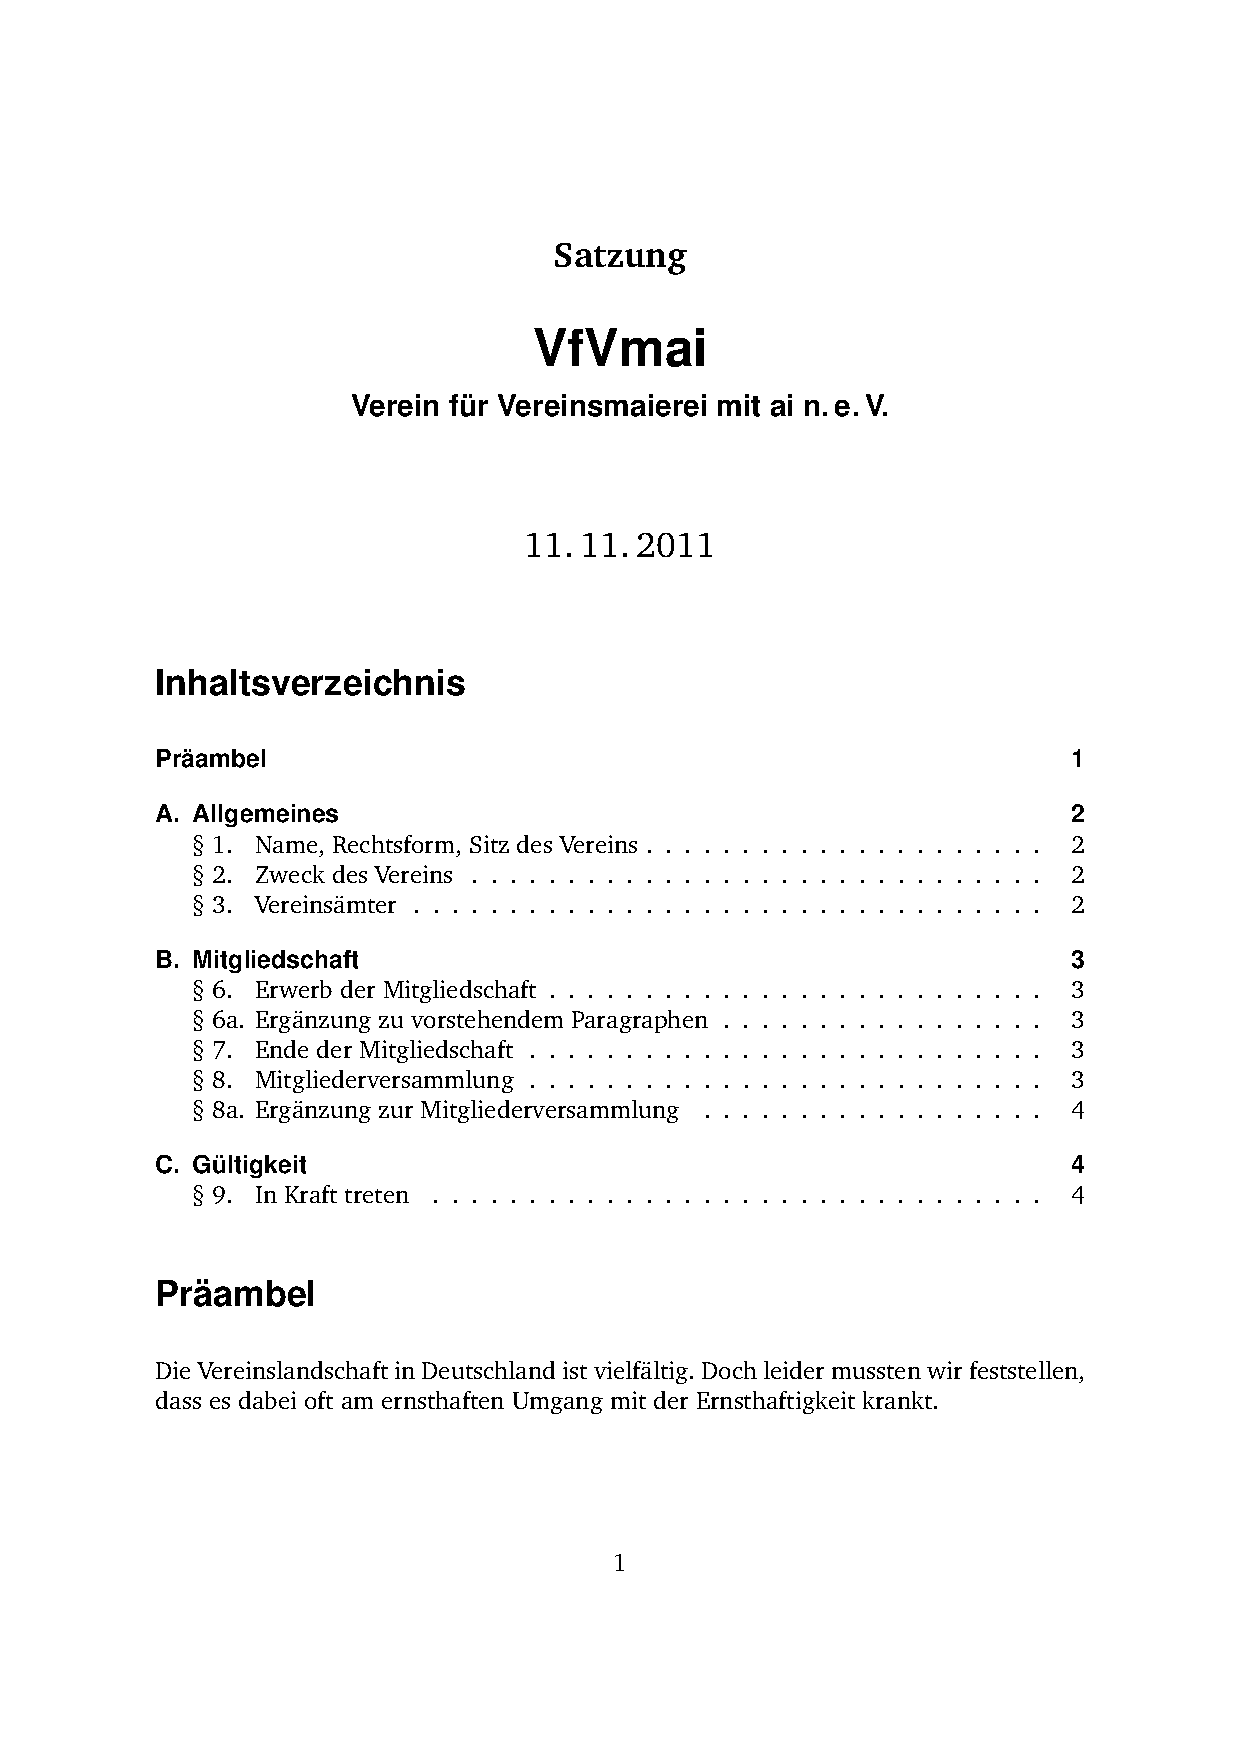
\includegraphics[page=1,width=.482\textwidth,%
        height=.49\textheight,keepaspectratio]{scrjura-example-de}}\enskip
      \frame{\includegraphics[page=2,width=.482\textwidth,%
        height=.49\textheight,keepaspectratio]{scrjura-example-de}}\par
      \smallskip}
    \begin{captionbeside}[{%
        Beispiel: Drei Seiten einer Beispielsatzung%
      }]{%
        Die ersten drei Seiten der Beispielsatzung aus
        \protect\autoref{sec:scrjura.example}%
      }%
      [l]
      \frame{\includegraphics[page=3,width=.482\textwidth,%
        height=.49\textheight,keepaspectratio]{scrjura-example-de}}\enskip
    \end{captionbeside}
  }{%
    {\hfill
      \frame{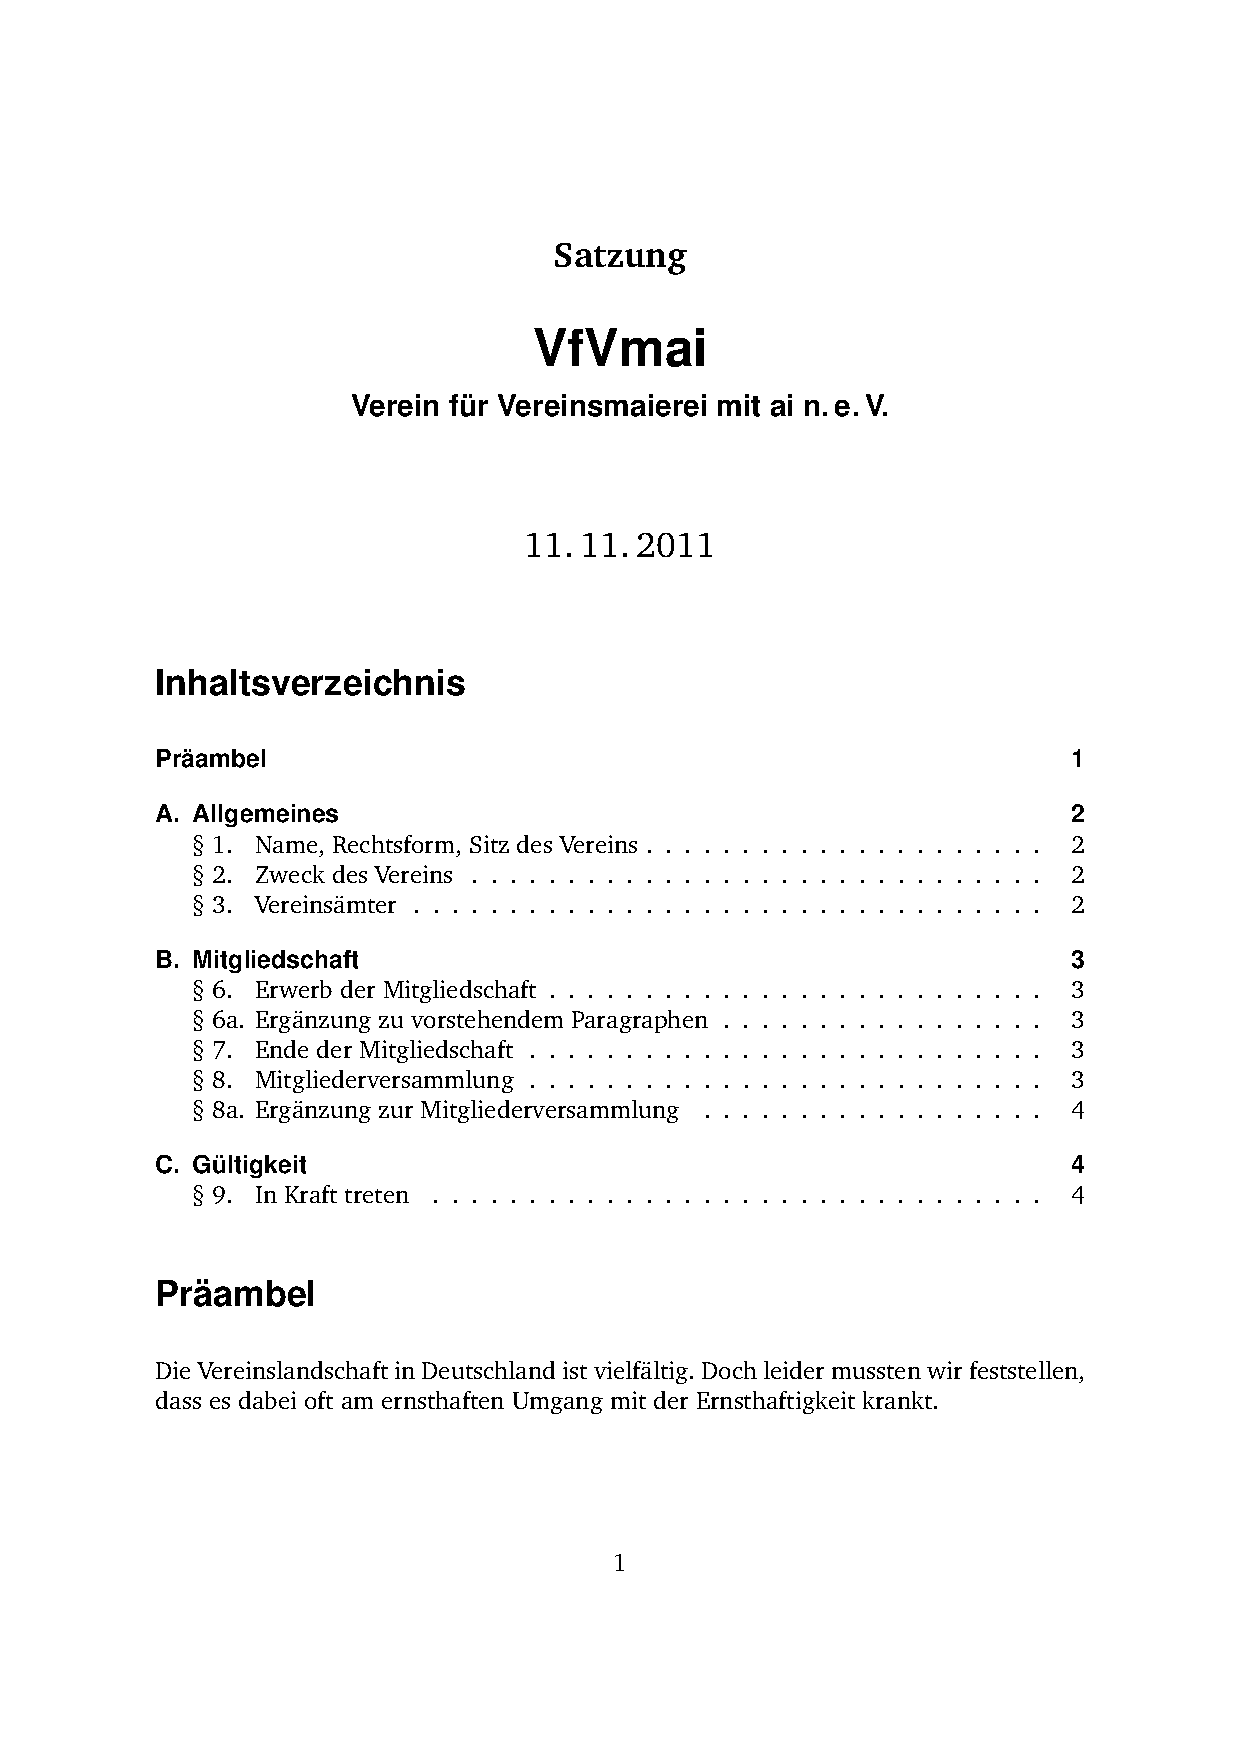
\includegraphics[page=1,width=.482\textwidth]{scrjura-example-de}}%
      \enskip
      \frame{\includegraphics[page=2,width=.482\textwidth]{scrjura-example-de}}\par
      \smallskip}
    \begin{captionbeside}[{%
        Beispiel: Drei Seiten einer Beispielsatzung%
      }]{%
        Die ersten drei Seiten der Beispielsatzung aus
        \protect\autoref{sec:scrjura.example}%
      }%
      [l]
      \frame{\includegraphics[page=3,width=.482\textwidth]{scrjura-example-de}}%
      \enskip
    \end{captionbeside}
  }%
  \label{fig:scrjura.example}
\end{figure}


\section{Entwicklungsstand}
\seclabel{draft}

Seit \KOMAScript~3.24 teilt \Package{scrjura} die Versionsnummer der Klassen
und anderer wichtiger Pakete. Dennoch sei auf einen wichtigen Punkt
hingewiesen: Bisher ist weder das Zusammenspiel mit vielen anderen Paketen
noch die Funktion der \DescRef{\LabelBase.env.contract}-Umgebung mit allen
möglichen \LaTeX-Umgebungen und Einstellungen verschiedener Klassen und Pakete
getestet. Dies liegt nicht zuletzt daran, dass es sich bei \Package{scrjura}
um ein sehr spezielles Paket handelt, das weit außerhalb der täglichen Praxis
des Autors liegt. Damit ist der Autor diesbezüglich in hohem Maße auf
ausführliche Rückmeldungen durch die Anwender angewiesen.%
\EndIndexGroup

%%% Local Variables: 
%%% mode: latex
%%% TeX-master: "scrguide-de.tex"
%%% coding: utf-8
%%% ispell-local-dictionary: "de_DE"
%%% eval: (flyspell-mode 1)
%%% End: 

% LocalWords:  Seitenstil bedarfsweise Ebenennummer Absatznummerierung
% LocalWords:  Paragraphenüberschrift Präambeln renewcommand Gesetzestexte
% LocalWords:  Grundgesetzartikel Absatzabstand umbrechbaren Wortabstand
% LocalWords:  Beispielsatzung Paragraphensymbol Vordefinierung Absatznummer
%  LocalWords:  Expandierbarkeit umbrechbarer Satznummer Paragraphenzeichen
